%%%% Better Poster latex template example v1.0 (2019/04/04)
%%%% GNU General Public License v3.0
%%%% Rafael Bailo
%%%% https://github.com/rafaelbailo/betterposter-latex-template
%%%% 
%%%% Original design from Mike Morrison
%%%% https://twitter.com/mikemorrison

\documentclass[a0paper,fleqn]{src/betterposter}

\begin{document}	
\betterposter{
%%%%%%%% MAIN COLUMN

\maincolumn{
%%%% Main space

\textbf{El espectrómetro por dentro}\\
\fontsize{75}{77}\selectfont % Set the font size to 12pt with a baseline skip of 14pt

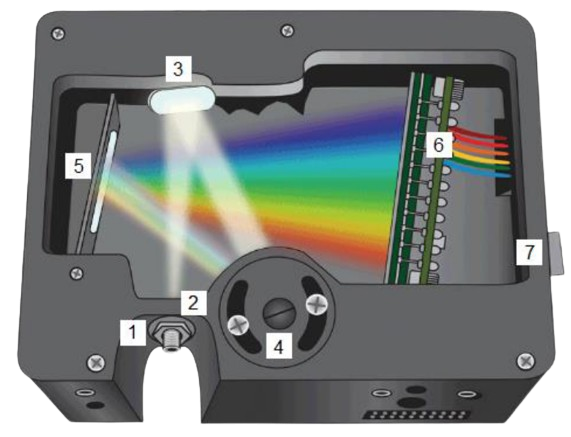
\includegraphics[width=\textwidth]{img/instrumento.png}\\

\vspace{-18cm}

}{
%%%% Bottom space

%% QR code
\qrcode{img/qrcode.png}{img/general/smartphoneBlack}{
\textbf{Fabrica tu propio espectrómetro} \\ Visita https:\slash \slash www.youtube.com \slash watch?v=023hmXZmGSc
}

}

}{
%%%%%%%% LEFT COLUMN

\title{Funcionamiento}
\author{Jorge Martinez}
\institution{Universidad Internacional de Valencia}

\section{\includegraphics[height=\fontcharht\font`\S]{img/general/slash.png} 1. Conector}
El conector redirige mediante fibra óptica la luz que recoge el telescopio.

\section{\includegraphics[height=\fontcharht\font`\S]{img/general/slash.png} 2. Entrada de luz}
El espectrografo comienza su funcionamiento cuando la luz incidente entra a
través de una rendija o una abertura en su extremo, lo que limita la cantidad de

\section{\includegraphics[height=\fontcharht\font`\S]{img/general/slash.png} 3. Collimación}
La luz entrante luego pasa a través de una lente colimadora. Esta lente tiene la
función de hacer que los rayos de luz sean paralelos, lo que facilita su
procesamiento en etapas posteriores.

\section{\includegraphics[height=\fontcharht\font`\S]{img/general/slash.png} 4. Dispersión}
La luz colimada incide en un prisma o una rejilla de difracción. Estos elementos
son los responsables de descomponer la luz en sus diferentes longitudes de onda,
lo que crea un patrón de dispersión. El prisma refracta la luz, mientras que la
rejilla de difracción la hace interferir de manera constructiva o destructiva,
separando las longitudes de onda.

\section{\includegraphics[height=\fontcharht\font`\S]{img/general/slash.png} 5. Enfoque}
Un espejo se encarga de enfocar las diferentes frecuencias en el sensor para su
posterior detección.


}{ % RIGHT COLUMN

\section{\includegraphics[height=\fontcharht\font`\S]{img/general/slash.png} 6. Detección}
El patrón de dispersión resultante se proyecta en una superficie detectora, como
un CCD (dispositivo de carga acoplada) o una película sensible a la luz. La
intensidad de la luz en cada punto del patrón se registra como una señal
eléctrica.

\section{\includegraphics[height=\fontcharht\font`\S]{img/general/slash.png} 7. Análisis de datos}
La señal eléctrica generada por el detector se convierte en un espectro mediante
un proceso de análisis de datos. Esto implica registrar la intensidad de la luz
a diferentes longitudes de onda y, a menudo, se realiza mediante un software
especializado.

\section{\includegraphics[height=\fontcharht\font`\S]{img/general/slash.png} 7. Interpretación del espectro}
El espectro resultante muestra picos o líneas que corresponden a las diferentes
longitudes de onda presentes en la luz original. Estos picos proporcionan
información valiosa sobre la composición química, la temperatura y otras
propiedades de la fuente de luz. 

\section{\includegraphics[height=\fontcharht\font`\S]{img/general/slash.png} 8. Poder de resolucion}
La resolución de un espectrómetro ($R$) nace de la rejilla de difracción y se
puede expresar mediante la ecuación $R = mN$, donde $R$ es la resolución, $m$ es
el orden de difracción y $N$ es el número de líneas por unidad de longitud en la
rejilla. Cuanto mayor sea $R$, mejor será la capacidad del espectrómetro para distinguir entre longitudes de onda cercanas. Además, el ángulo de incidencia ($\theta$) también influye en la resolución a través de la ecuación de la red de difracción de Bragg. 

}
\end{document}
